\documentclass[%
 reprint,
 amsmath,amssymb,
 aps,
]{revtex4-1}

\usepackage{graphicx}% Include figure files
\usepackage{dcolumn}% Align table columns on decimal point
\usepackage{bm}% bold math
\usepackage[dvipdfm,colorlinks=true,linkcolor=blue,filecolor=blue, urlcolor=blue]{hyperref}
\usepackage{braket}
\usepackage{caption} % captionsetup[figure]用
\usepackage{threeparttable} % Table のキャプションを変更
\usepackage{breqn} %dmath用：数式の自動折り返し
\numberwithin{equation}{section}% (p.37)

% \sloppy はすべての文章を「緩め」に設定し、オーバーフローや不均一な単語間隔を許すため、厳密な組版が求められる論文では推奨されません。
\tolerance=1000
\emergencystretch=1em
\hyphenpenalty=3000
\exhyphenpenalty=3000
\flushbottom
\usepackage[final]{microtype}


\begin{document}

    \captionsetup[figure]{justification=raggedright,
        labelfont={bf},name={Fig.},labelsep=period} %Fig.の注釈を左揃えするためrangedrightを用いる
    \captionsetup[table]{
        labelfont={bf},name={Table.},labelsep=period}

\title{Radiation-Mediated Quantum Tunneling:\\A Zitterbewegung Perspective}
\author{Satoshi Hanamura}
\email{hana.tensor@gmail.com}
    \date{December 14, 2024}
    %\date{\today}


\begin{abstract}
The Hartman effect—where quantum tunneling time remains invariant to barrier thickness—presents a fundamental paradox that challenges both classical physics and special relativity. Here, we introduce a theoretical framework that resolves this paradox by proposing a radiation-mediated energy transport mechanism coupled with the electron's Zitterbewegung oscillation occurring at four percent of light speed. Our model introduces a dual-kernel architecture where an electron's thermal potential energy simultaneously occupies two distinct spatial locations, providing a deterministic interpretation of quantum superposition and tunneling phenomena. During barrier traversal, we demonstrate that electrons undergo a particle-to-radiation transformation while kernel dissolution occurs over a duration corresponding to the time it takes to traverse the Compton wavelength at four percent of the speed of light, with radiation propagating at light speed over the Compton wavelength. Since the kernel dissolution period is long compared to the radiation propagation time, the overall tunneling duration remains effectively independent of barrier thickness. This theoretical framework accounts for both the Hartman effect and the experimentally verified absence of electrons within potential barriers, while maintaining consistency with both quantum mechanics and special relativity. Our findings recast quantum tunneling as a deterministic energy redistribution process, offering new insights into the fundamental nature of quantum phenomena while maintaining consistency with established physical principles.
\end{abstract}


\maketitle



\section{Introduction}
\label{sec:Introduction}

Quantum tunneling is a fundamental phenomenon of quantum mechanics, describing the ability of particles to overcome potential barriers despite lacking sufficient classical energy~\cite{griffiths2018, cohen2019}. Among its most enigmatic manifestations is the Hartman effect, where tunneling time remains nearly constant regardless of barrier thickness~\cite{hartman1962}. This behavior defies classical expectations and raises fundamental questions about its compatibility with special relativity~\cite{winful2006, buttiker1983}. While various approaches to redefining tunneling time have been proposed~\cite{buttiker1982, landauer1989}, challenges remain in developing a comprehensive theoretical framework.

This phenomenon manifests its fundamental importance across diverse applications, from facilitating nuclear fusion at reduced temperatures to enabling atomic-scale visualization through scanning tunneling microscopy~\cite{razavy2003, eigler1990}. However, the fundamental question of tunneling time—the duration required for particle traversal through a potential barrier—remains a important question that challenges our deepest understanding of quantum mechanics. Although seminal investigations~\cite{maccoll1932, hauge1989} illuminated the paradoxical nature of this process, contemporary experimental evidence continues to reveal fundamental limitations in the existing theoretical framework.

The Hartman effect, discovered in 1962~\cite{hartman1962}, reveals that beyond a certain barrier width, tunneling time becomes independent of the barrier’s thickness. This counterintuitive observation has sparked significant debate, as it appears to imply superluminal velocities, creating a conflict with the principles of special relativity~\cite{winful2006, buttiker1983}. Although various theoretical frameworks have attempted to address this paradox through alternative definitions of tunneling time~\cite{buttiker1982, landauer1989}, none have provided a comprehensive resolution that aligns fully with experimental observations and fundamental physics.

In this study, we introduce an approach based on the 0-Sphere model~\cite{hanamura2023}, which offers a fresh perspective on electron structure and dynamics. A proposed approach in our framework is the concept of thermal potential energy (TPE), which represents a fundamental departure from the classical notion of rest mass. In the 0-Sphere model, an electron's rest mass energy is not a static property but can transform into radiation energy during transport and reconstitute at a different location. This dynamic property of rest mass exists simultaneously at two distinct spatial locations in our dual-kernel structure. The cornerstone of our framework is this dual-kernel architecture, which not only challenges the conventional view of rest mass as a permanent, localized property but also provides a concrete physical basis for quantum superposition and tunneling phenomena. This interpretation not only provides a concrete physical basis for quantum superposition but also predicts a precise one-way transfer time of \( 2.00 \times 10^{-19} \, \mathrm{s} \) between the kernels, offering a theoretically derived timescale for quantum tunneling phenomena.

In contrast to previous methodologies based on wave packet analysis or perturbative techniques~\cite{steinberg1993, buttiker1982}, which frequently yield ambiguous interpretations of tunneling time, our approach employs closed algebraic equations centered on single-electron dynamics. The phenomena traditionally interpreted as quantum fluctuations within conventional quantum mechanics emerge in our framework as precise oscillations in thermal potential energy between the dual kernels, governed by explicit equations~\cite{darwin1928, breit1928}. This deterministic approach not only maintains consistency with the core principles of quantum mechanics but also provides a concrete, physically intuitive mechanism for tunneling phenomena.

The 0-Sphere model describes electron tunneling as an interconversion process between thermal potential energy (TPE) and kinetic energy. The TPE, which represents the electron's rest mass, transforms into thermal radiation and is treated as a kernel in this paper. This kernel rapidly converts to kinetic energy within approximately \( 2.00 \times 10^{-19} \, \mathrm{s} \). We shall refer to this as Kernel A.

Upon conversion of TPE to kinetic energy, this energy traverses the tunnel barrier through radiation transport. The radiation energy, after crossing the tunnel barrier, recondenses into TPE at a specific position, which we shall designate as Kernel B.

It is important to note that the positions of Kernel A and Kernel B are discrete. However, the kinetic energy transported via radiation from Kernel A to Kernel B exhibits wave-like properties and maintains continuity throughout the transport process.

This mechanism explains the Hartman effect and aligns with experimental findings that electrons are not observed within potential barriers~\cite{steinberg1993}, supporting the notion of radiation-mediated energy transfer. By maintaining consistency with both quantum mechanics and special relativity, this framework resolves the apparent paradox of superluminal tunneling velocities.

A distinctive feature of our approach is its divergence from traditional interpretations, as it formulates a geometrically precise quantum theory characterized by deterministic equations. By emphasizing the electron’s intrinsic oscillatory motion (Zitterbewegung)~\cite{breit1928, schrodinger1930} and its role in tunneling dynamics, we bridge the conceptual gap between quantum mechanics and classical intuition, offering a coherent explanation of the Hartman effect.

Our prior studies~\cite{hanamura2023} have demonstrated that Zitterbewegung, occurring at approximately four percent of the speed of light, explains the trembling motion of electrons. Historically dismissed as a mathematical artifact, this oscillatory behavior has gained experimental support~\cite{gerritsma2010, zawadzki2011}. The 0-Sphere model and the Dirac equation both describe this motion using first-order sine functions, revealing a mathematical correspondence between these distinct theoretical approaches.



\section{Theoretical Foundation: The Role of Rest Energy in Tunneling}
\label{sec:Theoretical Foundation}


To illustrate the theoretical framework, Fig.~\ref{f-tunnel} presents a comparative visualization. The conventional understanding of quantum tunneling, shown in Fig.~\ref{f-tunnel}a, depicts an evanescent wave decaying through a potential barrier. In contrast, the 0-Sphere model (Fig.~\ref{f-tunnel}b) introduces a fundamentally different mechanism: two spatially separated kernels ($A$ in green and $B$ in blue) connected through radiation pressure. The solid sinusoidal curve represents successful radiation-mediated transport where the electron has sufficient radiation energy to overcome the barrier, while the dashed curve shows the case of insufficient energy, both behaviors being analogous to a Slinky toy system's mechanical oscillations. The yellow arrow indicates the geodesic path of radiation energy transfer from kernel $A$ to kernel $B$, demonstrating how thermal potential energy is converted to radiation energy for barrier traversal. This mechanism provides a concrete physical interpretation for what has traditionally been described by evanescent waves in quantum mechanics.

\begin{figure}[t]
    \centering 
    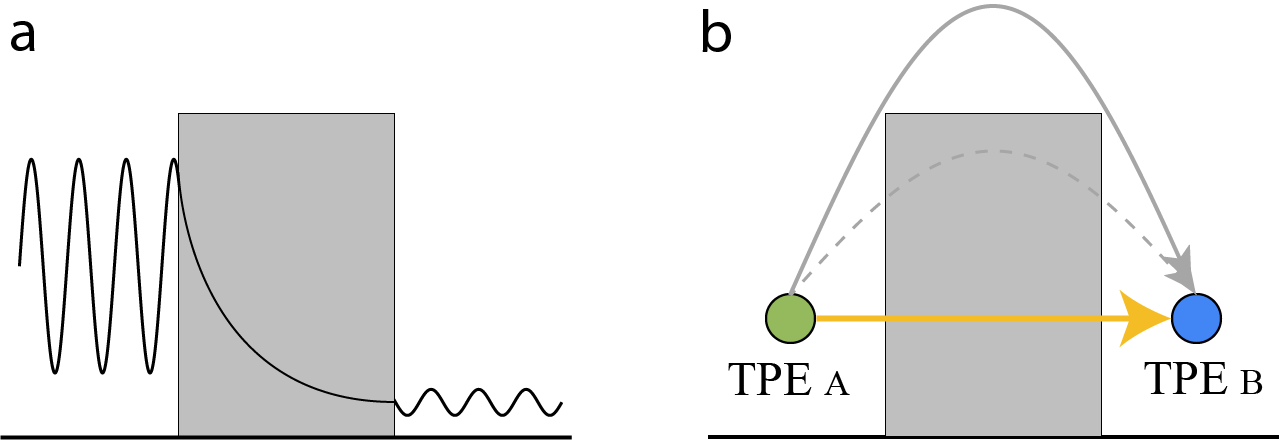
\includegraphics[scale=0.20]{f-tunnel.png}
    \caption{Comparison between conventional quantum tunneling and the proposed radiation-mediated transport mechanism. (a) Traditional representation showing an incident wave encountering a potential barrier and resulting in an evanescent wave. (b) The dual-kernel model showing kernels $A$ (green) and $B$ (blue) separated by a potential barrier. The solid sinusoidal curve represents successful radiation-mediated transport where the electron has sufficient radiation energy to overcome the barrier, while the dashed curve shows the case of insufficient energy for barrier traversal, both analogous to a mechanical Slinky toy system. The yellow arrow represents the geodesic path of radiation energy transfer between kernels, driven by radiation pressure---this geodesic trajectory, in the sense of general relativity, represents the actual path taken by the radiation energy. This mechanism transforms the abstract concept of quantum tunneling into a deterministic energy transport process between fixed kernel positions. The key point is that the kinetic energy of a single electron varies with its temporal phase. This result, derived from the 0-Sphere model, determines the probability of transmission or reflection depending on the temporal phase at which the electron collides with the tunnel barrier.}
    \label{f-tunnel}
\end{figure}


The fundamental of our analysis lies in understanding how an electron's rest energy ($E_0$) contributes to its tunneling behavior through periodic energy oscillations. A key concept in our framework is thermal potential energy (TPE), which represents the portion of rest energy that can be converted into radiation during the tunneling process. Unlike conventional potential energy, TPE characterizes the electron's capacity to exchange energy between its dual-kernel structure through thermal-radiative processes.

\begin{equation}
E_{0} = E_{0} \left( \cos^{4} \left( \frac{\omega t}{2} \right) + \sin^{4} \left( \frac{\omega t}{2} \right) + \frac{1}{2} \sin^{2} (\omega t) \right).
\label{eq:hamiltonian_expanded}
\end{equation}


\begin{figure}[t]
    \centering 
    
\includegraphics[scale=0.22]{f-total-hamiltonian.png}
    \caption{Energy distribution in the 0-Sphere model showing perfect energy conservation. The graph shows how energy oscillates between thermal and kinetic forms: thermal potential energy terms $\cos^4(\phi/2)$ at kernel $A$ and $\sin^4(\phi/2)$ at kernel $B$ (complementary oscillations), and kinetic energy term $(1/2)\sin^2(\phi)$ of the photon sphere (double-frequency oscillation). Their sum remains constant at 1 throughout the complete cycle of $4\pi$, demonstrating exact energy conservation as the system transitions between thermal potential and kinetic energy states.}
    \label{f-total-hamiltonian}
\end{figure}


This equation reveals the fundamental nature of electron behavior: a continuous interchange between thermal potential energy (TPE) and kinetic energy. The third term, $\frac{1}{2} \mathrm{sin}^{2} (\omega t)$, holds particular significance as it represents the oscillating component of the electron's kinetic energy, with a maximum amplitude of $\frac{1}{2}E_0$.

The radiation gradient in our electron model emerges from a precise mathematical relationship between two thermal potential energies (TPE). To understand its origin, let us examine how the TPE oscillates between two kernels:

\begin{equation}
    \mathrm{(TPE_A)}:T_{\mathrm{e1}} = E_0 \cos^4\left(\frac{\omega t}{2}\right),
    \label{eq:tpe_A}
\end{equation}
\begin{equation}
    \mathrm{(TPE_B)}:T_{\mathrm{e2}} = E_0 \sin^4\left(\frac{\omega t}{2}\right).
    \label{eq:tpe_B}
\end{equation}

Figure~\ref{f-total-hamiltonian} illustrates the perfect energy conservation in our electron model through the complementary oscillations of thermal and kinetic energies. When we examine the electron's motion between two kernels, we find that the TPE gradient drives a systematic energy conversion process. At point $A$, the electron possesses maximum thermal potential energy ($\cos^4(\phi/2)$ term peaks). As it moves toward point $B$, this TPE gradually converts into kinetic energy (represented by the $(1/2)\sin^2(\phi)$ term), driving the motion of the surrounding photon sphere. Upon reaching point $B$, the energy reconverts to TPE ($\sin^4(\phi/2)$ term peaks), and the process reverses. This oscillation maintains perfect energy conservation while enabling a unique form of periodic motion, as evidenced by the constant sum of all energy terms.

\begin{figure}[t]
    \centering 
    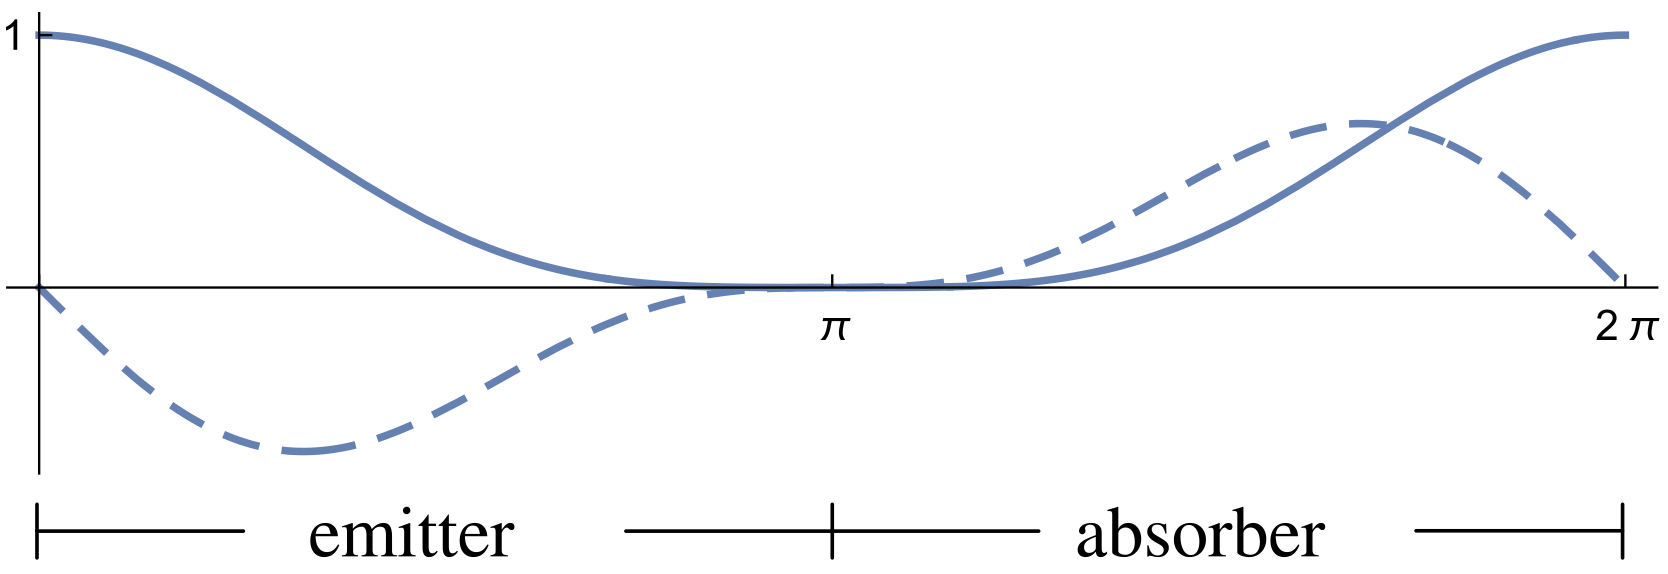
\includegraphics[scale=0.30]{f3_cos^4_cos^3.png}
    \caption{Time evolution of thermal potential energy (TPE) and its temporal derivative at kernel $A$. The solid line shows the TPE distribution ($\cos^4(\omega t/2)$), while the dashed line represents its temporal derivative ($ -2 \cos^{3} ( \omega t/2) \sin ( \omega t/2 )$), which corresponds to the radiation pressure driving the photon sphere. At temporal phase $\phi = \omega t = \pi$, ($\cos^4(\omega t/2)$) becomes zero, indicating that TPE at kernel $A$ completely vanishes. At this phase, all energy has been transferred to kernel $B$ ($\sin^4(\omega t/2)=1$), and the kinetic energy term $(1/2)\sin^2(\omega t)$ is also zero, signifying the completion of electron tunneling. The temporal derivative reveals how the radiation pressure changes over time, providing the mechanism for photon sphere propulsion between the kernels.}
    \label{f3_cos^4_cos^3}
\end{figure}

As shown in Fig.~\ref{f3_cos^4_cos^3}, the solid line represents how TPE at kernel $A$ varies with its temporal phase, while the dashed line shows its temporal derivative. The negative values of the temporal derivative up to $\omega t = \pi$ clearly indicate that kernel $A$ releases its TPE during this phase. This TPE gradient between points $A$ and $B$ provides the fundamental driving force for electron oscillation~\cite{hanamura2023}:

\begin{equation}
\operatorname{grad}(T_{\mathrm{e2}} - T_{\mathrm{e1}}) = E_0\sin(\omega t).
\label{eq:radiation_gradient}
\end{equation}

The resulting force emerges from the TPE difference between the two kernels. At kernel $A$, thermal energy is emitted through radiation, while at kernel $B$, this radiation is absorbed---creating a dynamic energy imbalance that propels the electron's motion. When the TPE is equal between the kernels, the photon sphere achieves its maximum velocity as all available thermal energy has been converted to kinetic energy. The sinusoidal form of the radiation gradient in Eq.~\ref{eq:radiation_gradient} behaves analogously to a spring-mass system: when the gradient reaches its maximum magnitude, it represents the state where the spring is either fully extended or fully compressed, exerting maximum force but yielding zero velocity of the attached mass. Similarly, when the TPE difference between kernels becomes zero ($(T_{e2} - T_{e1}) = 0$), the radiation gradient vanishes, corresponding to the moment when the photon sphere achieves its maximum velocity, just as a mass on a spring reaches peak velocity at the equilibrium point.

Based on these dynamics, periodic variations arise in the electron's kinetic energy, determining its ability to penetrate the barrier. The process begins at point $A$, where the electron possesses maximum thermal potential energy. As it moves toward the barrier, TPE converts to kinetic energy. The success of barrier penetration depends on whether the radiation energy reaches the threshold necessary to overcome the potential barrier. After penetration, kinetic energy reconverts to TPE at point $B$.

Through the gradient mechanism, periodic variations emerge in the electron's kinetic energy via light speed energy transfer between kernels. When encountering a potential barrier, the electron initially exists as a massive particle with maximum thermal potential energy at point $A$. As it reaches the barrier interface, this thermal potential energy converts to radiation energy. During barrier traversal, the energy propagates at light speed via the photon sphere, driven by radiation pressure gradients between the kernels. Upon emerging from the barrier, the radiation energy reconverts to thermal potential energy at point $B$, completing the tunneling process.


\section{Discussion}
\label{sec:discussion}

\subsection{Quantum Tunneling and Anomalous Magnetic Moment: A Unified Description}
\label{subsec:Quantum Tunneling and Anomalous}

The Hartman effect---which suggests that tunneling time remains invariant to barrier thickness—has been experimentally indicated. Through our theoretical framework that connects the electron's anomalous magnetic moment to its Zitterbewegung oscillation frequency, we can provide a quantitative explanation for this phenomenon. The quantum tunneling effect, as traditionally described by the Schrödinger equation, connects incident and transmitted waves through exponentially decaying functions within the potential barrier~\cite{cohen2019}.A fundamental connection between this conventional description and the 0-Sphere model lies in the nature of energy transmission through the barrier.

Experimentally, electrons cannot exist within the potential barrier itself---a fact that aligns with our model's fundamental premise that kernels $A$ and $B$ must be located outside the barrier region. In the 0-Sphere model, the transmitted wave corresponds to the kinetic energy of the photon sphere driven by radiation gradients generated between kernels $A$ and $B$. This correspondence provides an intuitive physical interpretation of the mathematical connection that the Schrödinger equation establishes between wavefunctions on either side of the barrier through exponential decay functions. To illustrate our model's mechanism of energy propagation through barriers (see Fig.~\ref{f-tunnel}b), a helpful analogy can be drawn from a familiar mechanical system.

Consider a Slinky toy moving along the $x$-axis between points $x = -a$ and $x = +a$, analogous to the sinusoidal trajectories shown in the figure. When we place a vertical barrier at $x = 0$, the Slinky's ability to traverse this barrier depends on its instantaneous dynamic state. This analog system helps illuminate how energy can propagate through a barrier via wave-like motion, similar to our model's radiation transport mechanism depicted by the solid and dashed curves in Fig.~\ref{f-tunnel}b.

\begin{figure}[t]
    \centering 
    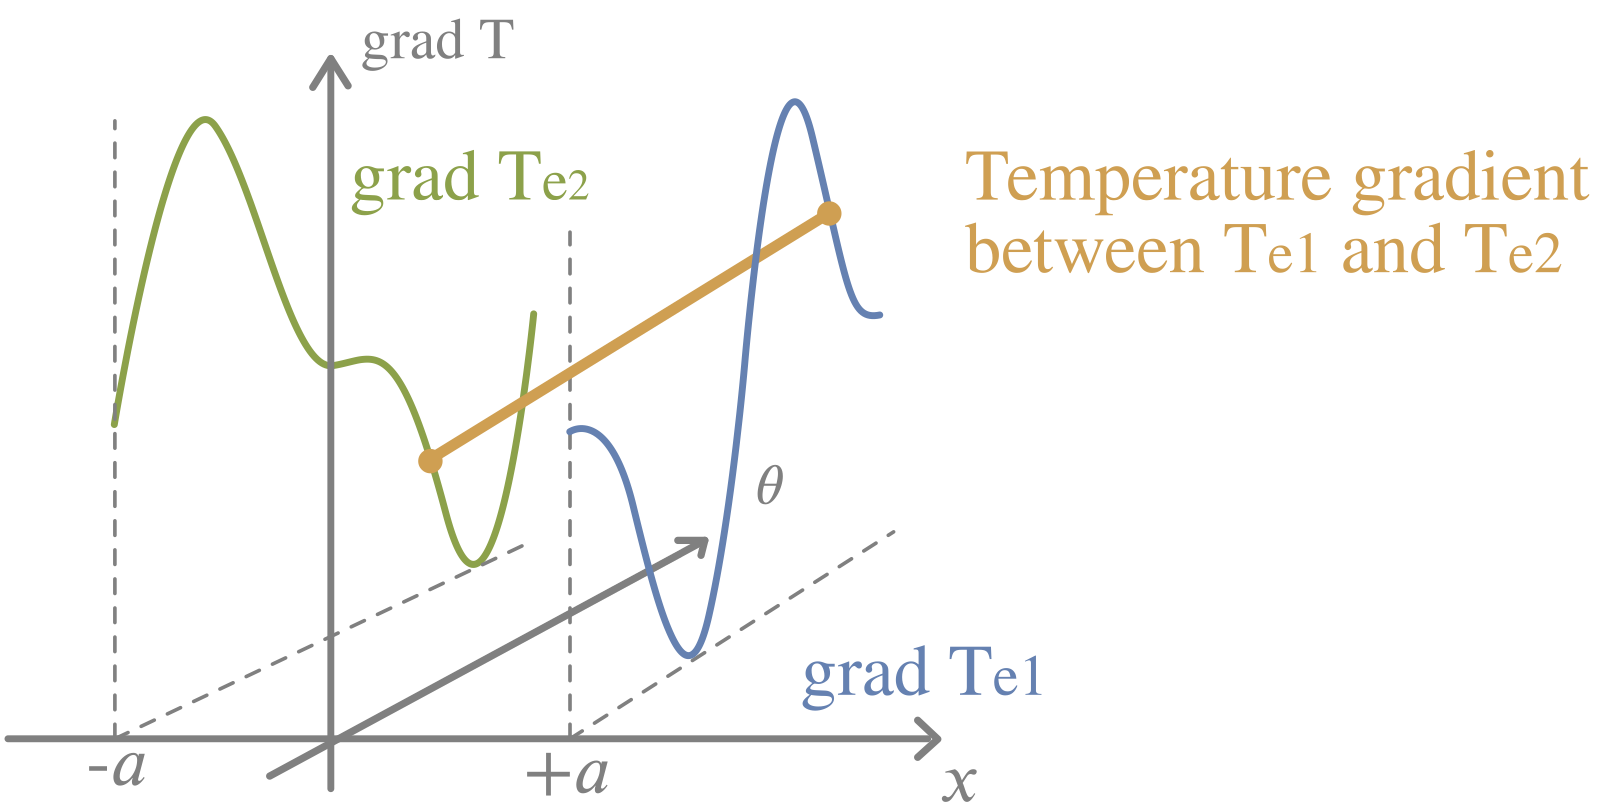
\includegraphics[scale=0.30]{f3_3D_temp_grad_^3.png}
    \caption{Spatial and temporal evolution of thermal gradients between two kernels. The blue and green curves show the individual thermal gradients (grad $T{e1}$ and grad $T{e2}$) at each kernel, while the orange line represents their difference (grad $(T{e2} - T{e1})$), which generates the radiation pressure driving the photon sphere. These gradients oscillate between points $-a$ and $+a$ with phase $\theta$, demonstrating how the radiation mechanism emerges from the coordinated behavior of both kernels.}
    \label{f3_3D_temp_grad_^3}
\end{figure}


The spatial and temporal evolution of the thermal gradients between kernels, visualized in Fig.~\ref{f3_3D_temp_grad_^3}, demonstrates how this radiation transport mechanism emerges from the coordinated behavior of both kernels. The gradient oscillations drive the photon sphere's motion, enabling energy to propagate through the barrier at light speed while maintaining total energy conservation. The radiation transport at light speed through the barrier leads to the apparent instantaneous tunneling characterized by the Hartman effect.

Our primary focus has been the Hartman effect, where tunneling time appears independent of barrier thickness. Let us synthesize our theoretical framework to address this phenomenon. In the 0-Sphere electron model, Zitterbewegung is not a mathematical artifact but rather an intrinsic oscillation of single electrons. This micro-oscillation should be experimentally verifiable, with an average velocity of approximately four percent of the speed of light. Given this constant average velocity, energy transfer between kernels $A$ and $B$ occurs through radiation transport, regardless of their separation distance. The transfer time corresponds to the period during which kernel $A$'s energy decreases from 100\% to 0\%, represented by the variation of $\cos^4(\phi/2)$ from 1 to 0 at four percent of light speed. This relationship determines the fundamental frequency of $\phi$.

An essential consideration is whether this average velocity is truly constant across all electrons. This is because the anomalous magnetic moment does not take on a different value for each electron. If this velocity varied between electrons, tunneling times would correlate with barrier thickness, or quantum mechanically speaking, might vary probabilistically between individual electrons. However, experimental observations consistently indicate a uniform velocity. Our research provides a deductive explanation for this constancy based on our previous findings. Zitterbewegung would be connected to the electron's anomalous magnetic moment through closed algebraic equations without relying on perturbation theory~\cite{hanamura2023}. The key equation relating the electron's micro-oscillation velocity to its anomalous magnetic moment is:

\begin{equation}
\sqrt{1 - \frac{v^2}{c^2}} = \frac{L}{L_0} = \frac{1}{1 + \frac{1}{\sqrt{2}}a^{\text{exp}}_{\text{e}}} ,
\label{eq:new5}
\end{equation}
where $v$ represents the average velocity due to Zitterbewegung, $c$ is the speed of light, and the ratio $L/L_0$ represents the Lorentz contraction factor. Here, $L_0$ represents the length measured by an external observer when viewing the electron from outside (where the anomalous magnetic moment is observable), while $L$ is the contracted length that would be measured from a reference frame moving with the electron's Zitterbewegung motion. This distinction is crucial because, as our thought experiment suggests, an observer hypothetically located inside the electron would measure exactly $g=2$, as predicted by the Dirac equation. Notably, this equation serves as the theoretical foundation for our prediction that the electron's Zitterbewegung velocity is approximately four percent of the speed of light---a value that emerges directly from substituting the experimental value of the anomalous magnetic moment into Eq.~\ref{eq:new5}. The experimental value of the anomalous magnetic moment is precisely known~\cite{Fan}:

\begin{equation}
a^{\text{exp}}_{\text{e}}=0.001\,159\,652\,180\,59\,(13) .
\label{eq:anomalous}
\end{equation}

Substituting the experimental value of the electron's anomalous magnetic moment given in Eq.~\ref{eq:anomalous} into Eq.~\ref{eq:new5}, we obtain:
\begin{align}
\sqrt{1 - \frac{v^2}{c^2}} &= \frac{1}{1 + \frac{1}{\sqrt{2}}(0.001\,159\,652\,180\,59)} \nonumber \\
&\approx 0.999\,179 \nonumber
\end{align}
Therefore,
\begin{align}
1 - \frac{v^2}{c^2} &\approx 0.998\,359 \nonumber \\
\frac{v^2}{c^2} &\approx 0.001\,641 \nonumber \\
\frac{v}{c} &\approx 0.040\,506 \nonumber
\end{align}
Thus, we obtain a value of $v$ that is approximately four percent of the speed of light.

Equation~\ref{eq:new5} establishes a fundamental relationship between electron micro-oscillation velocity and the anomalous magnetic moment. It implies that if the anomalous magnetic moment is constant, the micro-oscillation velocity must also be constant. The period during which $\cos^4(\phi/2)$ varies from 1 to 0 corresponds to $\phi = \pi$, as $\cos(\phi/2)$ becomes zero at $\phi/2 = \pi/2$. Given that this variation occurs at four percent of light speed and involves a distance of one Compton wavelength $\lambda_c = h/(m_ec) = 2.43 \times 10^{-12}$ m, we can calculate the corresponding time period:
\begin{equation}
\begin{aligned}
T &= \frac{\lambda_c}{0.0405c} \
&= \frac{2.43 \times 10^{-12}}{0.0405 \cdot 3.00 \times 10^8} \
&\approx 2.00 \times 10^{-19} \mathrm{s}.
\label{eq:period}
\end{aligned}
\end{equation}
From this period, the angular frequency is derived as:
\begin{equation}
\omega = \frac{2\pi}{T} \approx 3.14 \times 10^{19} \mathrm{rad/s}.
\label{eq:frequency}
\end{equation}
Consequently, the corresponding frequency becomes:
\begin{equation}
f = \frac{\omega}{2\pi} \approx 5.00 \times 10^{18} \mathrm{Hz}.
\label{eq:natural_frequency}
\end{equation}
These precise numerical predictions---particularly the characteristic frequency of $5.00 \times 10^{18}$ Hz---emerge naturally from our theoretical framework. While direct experimental verification of this high-frequency oscillation remains a significant challenge for current measurement techniques, the internal consistency of our analysis provides a clear resolution to the Hartman effect: the constancy of tunneling time arises from electrons traversing potential barriers through micro-oscillations, whose velocity remains uniform across all electrons due to the universality of the anomalous magnetic moment.

Direct experimental verification of this high-frequency oscillation remains a significant challenge for current measurement techniques. However, our analysis provides a clear resolution to the Hartman effect: the constancy of tunneling time arises from electrons traversing potential barriers through micro-oscillations, whose velocity remains uniform across all electrons due to the universality of the anomalous magnetic moment.

This cyclic transformation provides a physical mechanism for quantum fluctuations described in traditional quantum theory. When an electron encounters a potential barrier, the thermal potential energy converts to radiation energy, allowing the electron to traverse the barrier region as pure energy rather than as a massive particle. This mechanism explains both the tunneling process and the experimental observation that electrons are never detected within potential barriers.

The present theoretical framework requires further development to address quantum tunneling effects in the critical energy range of approximately 1-100 eV, where these phenomena predominantly occur. A comprehensive analysis must examine how applied voltage in this range influences both the electron's dual-kernel structure and the energy transfer mechanisms between kernels. Understanding these interactions would validate the theoretical framework while advancing our capacity to predict and control quantum tunneling in practical applications. Future investigations should focus on incorporating voltage-dependent behaviors and their effects on the energy redistribution process, thereby strengthening the connection between theoretical predictions and experimental observations.


\section{Conclusion}
\label{sec:Conclusion}

This study introduces a theoretical framework that could provide a clue about quantum tunneling through a radiation-mediated transport mechanism between two spatially separated kernels. By establishing a direct connection between electron Zitterbewegung and the anomalous magnetic moment, our proposed model offers a possible explanation for the Hartman effect---the phenomenon where tunneling time remains constant regardless of barrier thickness. This connection demonstrates that the constancy of tunneling time is a natural consequence of the universal value of the electron's anomalous magnetic moment. In conventional quantum theory, electrons are treated as wave packets, leading to problematic discussions of group velocity and potential superluminal transmission. Instead, we adopt a deterministic approach based on our previous prediction that electron Zitterbewegung occurs at approximately four percent of light speed, providing a natural explanation for the velocity independence of tunneling.

The proposed approach lies in the dual-kernel structure, where an electron's thermal potential energy simultaneously exists at two distinct locations, connected by a radiation field that enables energy transfer with a precisely calculated transfer time of $\mathrm{s} \approx 2.00 \times 10^{-19} \, \mathrm{s}$ (Eq.~\ref{eq:period}). This characteristic time approximately corresponds to the duration required for traversing the electron's Compton wavelength at four percent of light speed, providing a fundamental physical basis for our model. The mathematical formalism developed here applies our previous prediction of Zitterbewegung frequency $f = 5.00 \times 10^{18} \, \mathrm{Hz}$ (Eq.~\ref{eq:natural_frequency}) to quantum tunneling phenomena, with this characteristic frequency emerging naturally from the fundamental equations of our model.

The disappearance of kernels is not instantaneous but occurs over a finite period of $\mathrm{s} \approx 2.00 \times 10^{-19}  \mathrm{s}$, corresponding to the time it takes to traverse the Compton wavelength at four percent of the speed of light. During this period, radiation transport of rest mass continues between the kernels. This transfer time, as given by Eq.~\ref{eq:period}, characterizes the period of sustained radiation exchange between the kernels. This dual process, where kernel dissolution occurs while maintaining continuous radiation transport, suggests not only an internal structure of electrons but also their finite spatial extent, while the radiation traverses the tunnel barrier at light speed. Since this kernel dissolution period is approximately 25 times longer than (calculated as 1/0.04) the light-speed transmission time through the barrier, this mechanism explains the experimental observation that tunneling time remains constant regardless of barrier thickness.

This model could contribute to understanding in physics. For instance, the Schrödinger equation operates in absolute time, whereas the 0-Sphere model assigns individual angular velocities to each electron. This enables the application of proper time concepts from general relativity to individual electrons. Furthermore, if electron transport fundamentally occurs through radiation transmission of rest mass, Snell's law becomes applicable. This could serve as an initial step in bridging quantum mechanics and general relativity. While our theoretical framework presents a mathematical framework, further experimental investigations are needed to validate these predictions, particularly regarding the precise measurement of radiation-mediated energy transfer during tunneling events.

% \vspace{2cm} % 2cmの垂直空白を追加

% = = * * = =  * * = = * * = = * * = = * * = = * * = = * * = = * * 

\begin{thebibliography}{99}

\bibitem{griffiths2018}
Griffiths, D. J.,
\textit{Introduction to Quantum Mechanics},
Cambridge University Press, 3rd Edition (2018).

\bibitem{cohen2019}
Cohen-Tannoudji, C., Diu, B., \& Laloë, F.,
\textit{Quantum Mechanics},
Wiley-VCH, 3rd Edition (2019).

\bibitem{hartman1962}
Hartman, T. E.,
\textit{Tunneling of a wave packet},
Journal of Applied Physics \textbf{33}, 3427-3433 (1962),
\href{https://doi.org/10.1063/1.1702424}{doi:10.1063/1.1702424}.

\bibitem{winful2006}
Winful, H. G.,
\textit{Tunneling time, the Hartman effect, and superluminality: A proposed resolution of an old paradox},
Physics Reports \textbf{436}, 1-69 (2006),
\href{https://doi.org/10.1016/j.physrep.2006.09.002}{doi:10.1016/j.physrep.2006.09.002}.

\bibitem{buttiker1983}
Büttiker, M.,
\textit{Hartman effect and non-locality in quantum networks},
Physical Review B \textbf{27}, 6178 (1983),
\href{https://doi.org/10.1103/PhysRevB.27.6178}{doi:10.1103/PhysRevB.27.6178}.

\bibitem{buttiker1982}
Büttiker, M. \& Landauer, R.,
\textit{Traversal Time for Tunneling},
Physical Review Letters \textbf{49}, 1739-1742 (1982),
\href{https://doi.org/10.1103/PhysRevLett.49.1739}{doi:10.1103/PhysRevLett.49.1739}.

\bibitem{landauer1989}
Landauer, R.,
\textit{Barrier traversal time},
Nature \textbf{341}, 567-568 (1989),
\href{https://doi.org/10.1038/341567a0}{doi:10.1038/341567a0}.

\bibitem{razavy2003}
Razavy, M.,
\textit{Quantum Theory of Tunneling},
World Scientific Publishing Company (2003),
\href{https://doi.org/10.1142/5155}{doi:10.1142/5155}.

\bibitem{eigler1990}
Eigler, D. M. \& Schweizer, E. K.,
\textit{Positioning single atoms with a scanning tunnelling microscope},
Nature \textbf{344}, 524-526 (1990),
\href{https://doi.org/10.1038/344524a0}{doi:10.1038/344524a0}.

\bibitem{hauge1989}
Hauge, E. H. \& Støvneng, J. A.,
\textit{Tunneling times: a critical review},
Reviews of Modern Physics \textbf{61}, 917-936 (1989),
\href{https://doi.org/10.1103/RevModPhys.61.917}{doi:10.1103/RevModPhys.61.917}.

\bibitem{maccoll1932}
MacColl, L. A.,
\textit{Note on the Transmission and Reflection of Wave Packets by Potential Barriers},
Physical Review \textbf{40}, 621-626 (1932),
\href{https://doi.org/10.1103/PhysRev.40.621}{doi:10.1103/PhysRev.40.621}.

\bibitem{hanamura2023}
S. Hanamura, Redefining Electron Spin and Anomalous Magnetic Moment Through Harmonic Oscillation and Lorentz Contraction, Zenodo (2023), \href{https://doi.org/10.5281/zenodo.17764997}{doi:10.5281/zenodo.17764997}. [Originally: \href{https://vixra.org/abs/2309.0047}{viXra:2309.0047}]

\bibitem{steinberg1993}
Steinberg, A. M., Kwiat, P. G. \& Chiao, R. Y.,
\textit{Measurement of the single-photon tunneling time},
Physical Review Letters \textbf{71}, 708-711 (1993),
\href{https://doi.org/10.1103/PhysRevLett.71.708}{doi:10.1103/PhysRevLett.71.708}.

\bibitem{breit1928}
Breit, G.,
\textit{An Interpretation of Dirac's Theory of the Electron},
Proceedings of the National Academy of Sciences \textbf{14}, 553-559 (1928),
\href{https://doi.org/10.1073/pnas.14.7.553}{doi:10.1073/pnas.14.7.553}.

\bibitem{darwin1928}
Darwin, C. G.,
\textit{The wave equations of the electron},
Proceedings of the Royal Society A \textbf{118}, 654-680 (1928),
\href{https://doi.org/10.1098/rspa.1928.0076}{doi:10.1098/rspa.1928.0076}.

\bibitem{schrodinger1930}
Schrödinger, E.,
\textit{Über die kräftefreie Bewegung in der relativistischen Quantenmechanik},
Sitzungsberichte der Preussischen Akademie der Wissenschaften \textbf{24}, 418-428 (1930),
\href{https://doi.org/10.1002/3527608842.ch28}{doi:10.1002/3527608842.ch28}.

\bibitem{gerritsma2010}
Gerritsma, R., Kirchmair, G., Zähringer, F., Solano, E., Blatt, R., \& Roos, C. F.,
\textit{Quantum simulation of the Dirac equation},
Nature \textbf{463}, 68-71 (2010),
\href{https://doi.org/10.1038/nature08688}{doi:10.1038/nature08688}.

\bibitem{zawadzki2011}
Zawadzki, W., \& Rusin, T. M.,
\textit{Zitterbewegung (trembling motion) of electrons in semiconductors: a review},
Journal of Physics: Condensed Matter \textbf{23}, 143201 (2011),
\href{https://doi.org/10.1088/0953-8984/23/14/143201}{doi:10.1088/0953-8984/23/14/143201}.

%\bibitem{hanamura2018}
%S. Hanamura, A Model of an Electron Including Two Perfect Black Bodies, Zenodo (2018), \href{https://doi.org/10.5281/zenodo.16759284}{doi:10.5281/zenodo.16759284}. [Originally: \href{https://vixra.org/abs/1811.0312}{viXra:1811.0312}]

\bibitem{Fan}
Fan, X., Myers, T. G., Sukra, B. A. D. \& Gabrielse, G., Measurement of the Electron Magnetic Moment, Phys. Rev. Lett. \textbf{130}, no.7, 071801 \href{https://arxiv.org/abs/2209.13084}{arXiv:2209.13084} (2023)

\end{thebibliography}

% = = * * = =  * * = = * * = = * * = = * * = = * * = = * * = = * * 
% \section{\label{sec:Appendix}Appendix}

% \section*{Acknowledgments}

\end{document}

